 The algorithms and methods discussed in the previous chapters for preprocessing, feature extraction and classification are implemented as a configurable brain signal processing pipeline. This chapter provides analysis of the results obtained from BCI signal processing pipeline combining different preprocessing, feature extraction and classification algorithms with data from OpenBCI headgear. Several open source libraries were used in BCI data extraction, analysis and visualization. Metrics such as accuracy, F1, Receiver Operating Characteristics (ROC) and cross validation time for the Machine Learning methods were used to analyse the results and used to control the simulated car in CARLA.

\section{Tools}
\subsection{OpenBCI headgear}
OpenBCI is an open-source BCI platform that develops hardware and software for BCI scientific research. It provides electrodes, interface boards, graphical user interface and python API. In this work, the OpenBCI system consists of a 3D printed headgear with 16 EEG electrodes connected to Cython + Daisy board that interacts to the host machine wireless through an external dongle via serial communication. Cython is a 8-channel neural interface with a 32-bit processor which has a sampling frequency of 250 Hz. It is topped with Daisy, an extension board which can add up to 8 more channels to the system. This leads to drop in the sampling frequency to 125 HZ. With a WiFi module it is possible to achieve 1000 Hz. The potential difference between the electrodes and the reference points such as linked mastoids, inion or nasion. The measurements can be visualized on the host machine using OpenBCI GUI. The electrodes are placed in the internationally recognized 10-20 system. The measurement data can be streamed to the work station through BrainFlow or LSL. 

\subsection{CARLA}
CARLA \cite{2017_Carla} is an open-source simulator to develop, train and validate autonomous driving systems. It supports ROS for establishing communication between CARLA server and clients that can feed into or extract data from the CARLA environment.

\subsection{MNE}
MNE \cite{2013_MNE} is an open-source python package for exploring, visualizing and analyzing neuro-physiological data. It provides support for various preprocessing, feature extraction and classification steps in brain signal analysis.

\section{Experiment setup} 
With the tools discusses above, a working model of the BCI system could be established. The measurements from the OpenBCI headgear are transferred to the workstation with OpenBCI GUI through serial communication. This information is then transferred to the BCI classifier ROS package where preprocessing such as CAR, ICA, SSP are applied to remove the artifacts, features are extracted and classified according to the motor intent. The classified motor action is sent as steering command to CARLA through the CARLA-ROS bridge. 

During the training phase (see figure \ref{fig:exp_third_person_view2}), the EEG data from the OpenBCI headgear is epoched for 12 seconds and used as training data for the BCI pipeline. The training environment consists of a vertical line that changes color in the beginning of each trial. The yellow square provides motor intent instruction that needs to be performed by the user. The training can be both online and offline. In case of online training, the measurement are preprocessed, features are extracted, classified and the system is trained along with the ground truth information. The feedback to the user is provided with the help of a grey square that moves to direction of the classified motor intent. In offline training, the data is measured, stored along with the ground truth information, which is later used in training the system.

     \begin{figure}[H]
        \begin{center}
        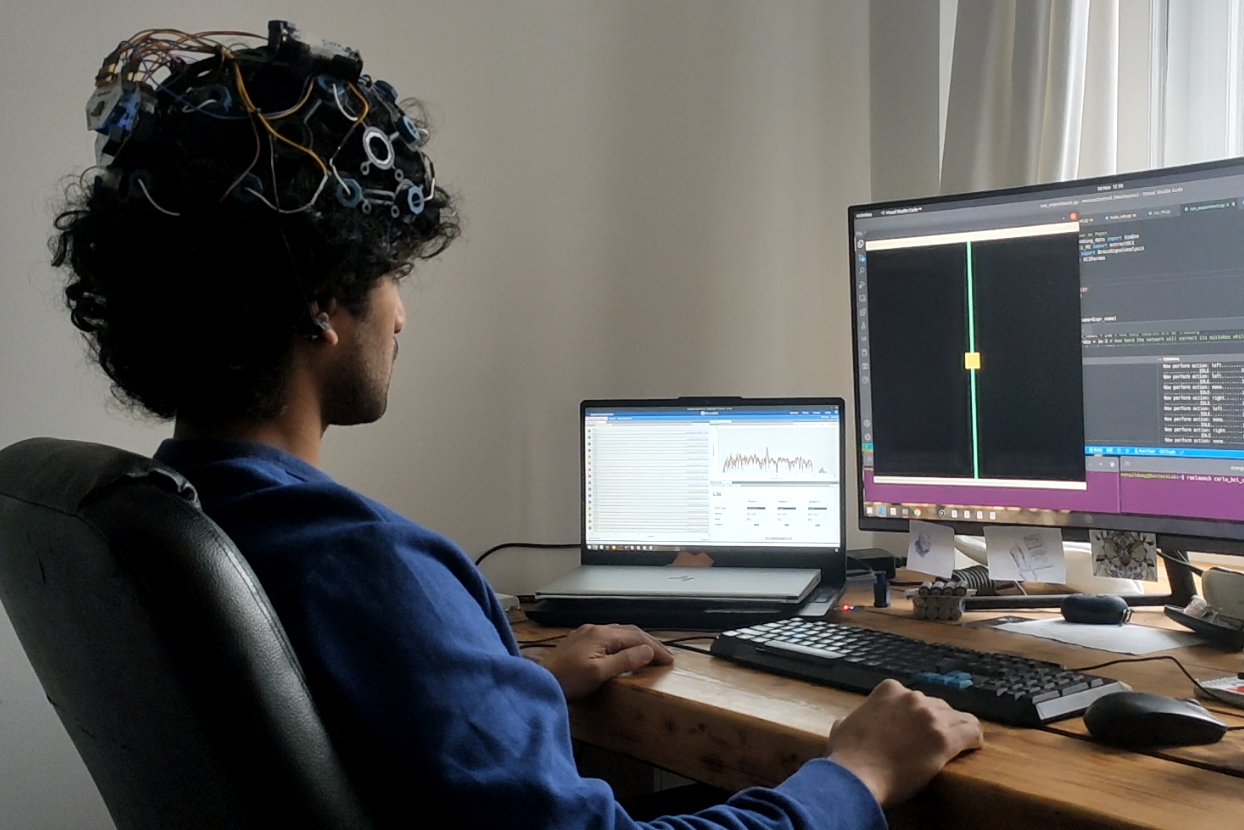
\includegraphics[width=1.0\textwidth]{images/exp_third_person_view2.png}
        \caption{Third person view of a user with the BCI system in training phase}
        \label{fig:exp_third_person_view2}
        \end{center}
    \end{figure}

During the testing phase (see figure \ref{fig:exp_third_person_carla1}), the trained system is deployed to control the steering of the simulated car in CARLA.

     \begin{figure}[H]
        \begin{center}
        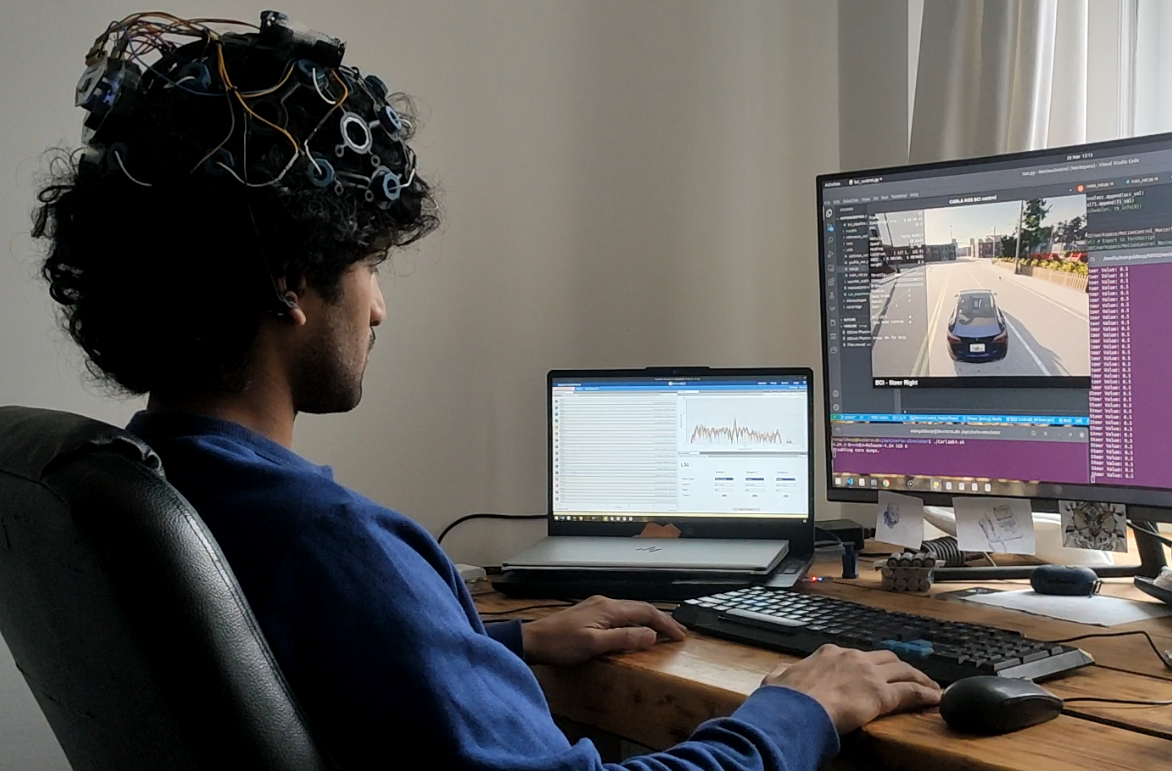
\includegraphics[width=1.0\textwidth]{images/exp_third_person_carla1.png}
        \caption{Third person view of a user with the BCI system in testing phase}
        \label{fig:exp_third_person_carla1}
        \end{center}
    \end{figure}

The figures \ref{fig:carla_left}, \ref{fig:carla_neutral}, \ref{fig:carla_right} show the simulated car controlled by the motor intent of the user. It can be observed in figure \ref{fig:carla_right} that the vehicle had left the lane while performing a right turn. This is because of epoching the measurement for 12 seconds, leading to a delay of conveying the command to CARLA.

     \begin{figure}[H]
        \begin{center}
        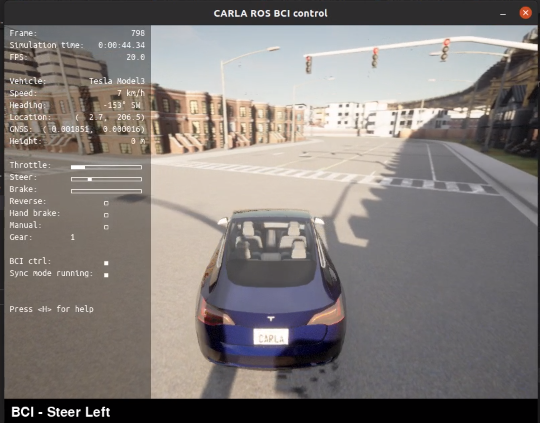
\includegraphics[width=1.0\textwidth]{images/carla_left1.png}
        \caption{Car taking a left with the command decoded from the motor intent.}
        \label{fig:carla_left}
        \end{center}
    \end{figure}

     \begin{figure}[H]
        \begin{center}
        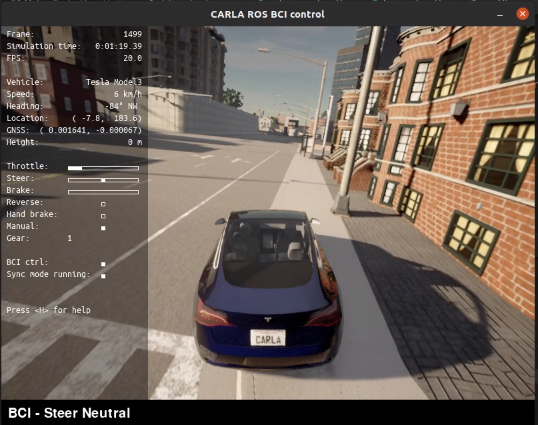
\includegraphics[width=1.0\textwidth]{images/carla_neutral1.png}
        \caption{Car driving straight with the command decoded from the motor intent.}
        \label{fig:carla_neutral}
        \end{center}
    \end{figure}

     \begin{figure}[H]
        \begin{center}
        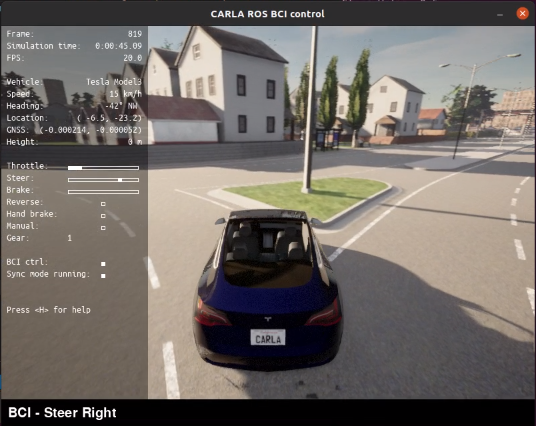
\includegraphics[width=1.0\textwidth]{images/carla_right1.png}
        \caption{Car taking a right with the command decoded from the motor intent.}
        \label{fig:carla_right}
        \end{center}
    \end{figure}
    
\section{Preprocessing}
 The preprocessing steps chosen are dependent on the datasets used. Artifact removal is the first process performed on any dataset. The figure \ref{fig:test_acc} and \ref{fig:test_f1} shows the influence of different preprocessing steps for various feature extraction techniques and its combinations in the test accuracy and F1 score respectively. 

     \begin{figure}[H]
        \begin{center}
        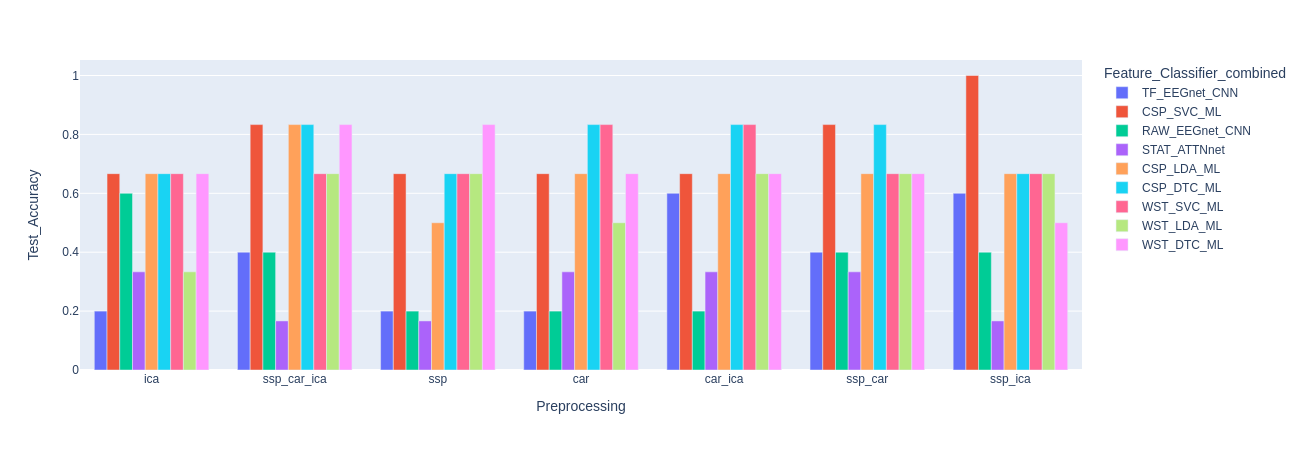
\includegraphics[width=1.0\textwidth]{images/preproc_test_acc_feat_bar.png}
        \caption{Accuracy for different preprocessing methods}
        \label{fig:test_acc}
        \end{center}
    \end{figure}

Although all the preprocessing steps, produce very similar results, It can be seen that ICA and SSP reduces the variance in the results and has higher median. CAR records the highest variance for several combinations of feature extraction and classifiers. The F1 score and test accuracy provide very similar results.

     \begin{figure}[H] 
     \begin{center}
        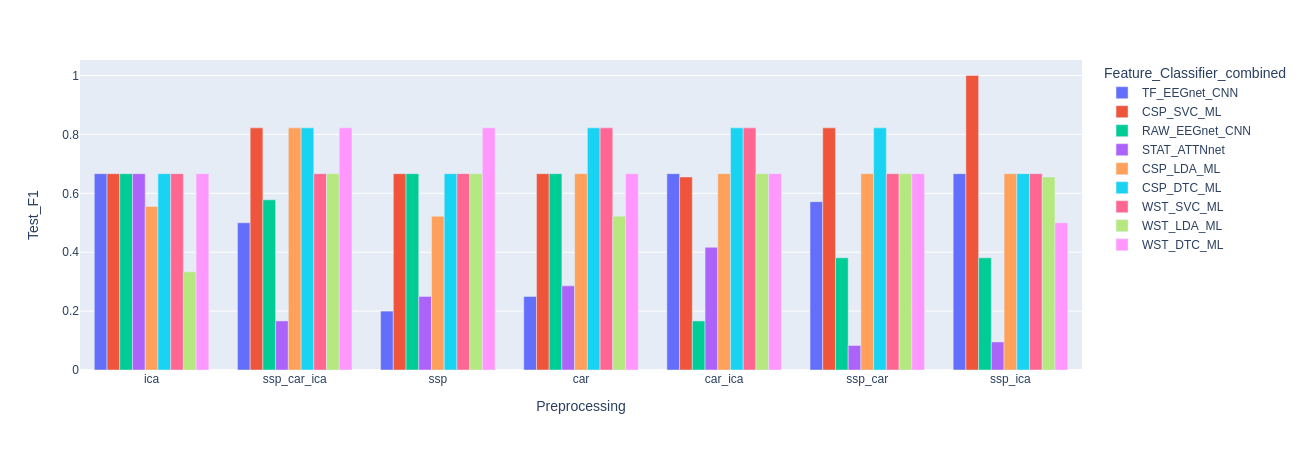
\includegraphics[width=1.0\textwidth]{images/preproc_test_f1_feat_bar.png}
        \caption{F1 score for different preprocessing methods}
        \label{fig:test_f1}
    \end{center}    
    \end{figure}

\section{Feature Extraction}
Features such as CSP, WST coefficients, statistics, time-frequency values were used, apart from raw measurement data after the preprocessing steps. The test accuracy \ref{fig:preproc_test_acc_features} and test f1 score \ref{fig:preproc_test_f1_features} are compared for the analysis with different preprocessing steps.
     \begin{figure}[H] 
     \begin{center}
        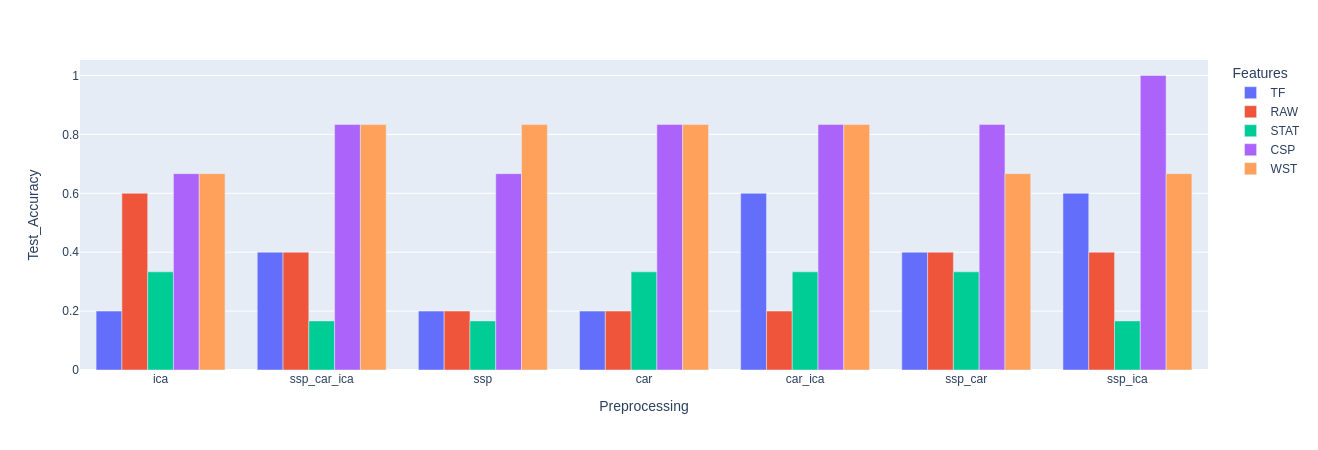
\includegraphics[width=1.0\textwidth]{images/preproc_test_acc_features_bar.png}
        \caption{Accuracy for different feature extraction methods}
        \label{fig:preproc_test_acc_features}
        \end{center}
    \end{figure}

     \begin{figure}[H] 
     \begin{center}
        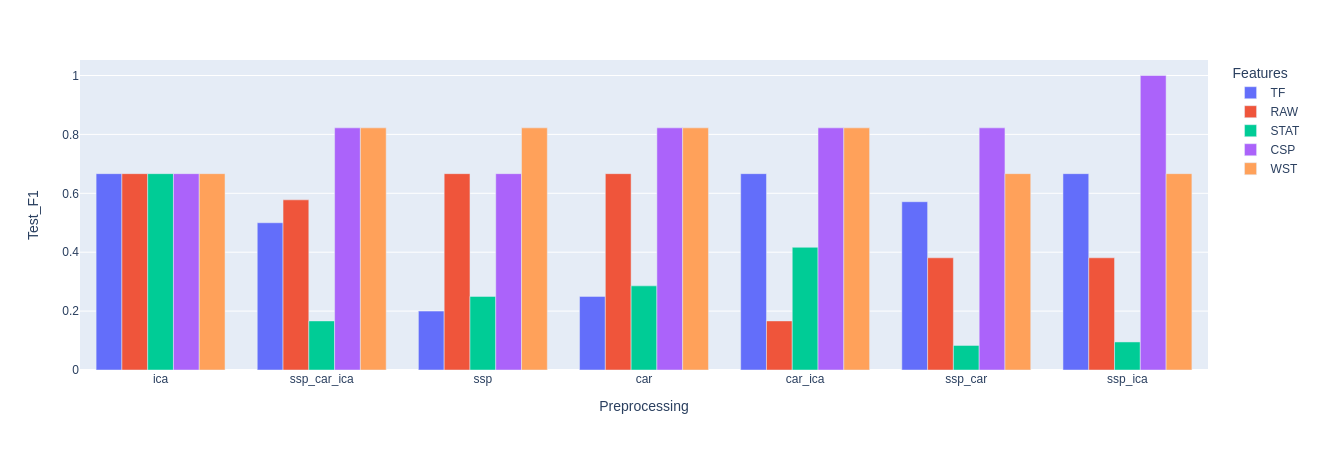
\includegraphics[width=1.0\textwidth]{images/preproc_test_f1_features_bar.png}
        \caption{F1 score for different feature extraction methods}
        \label{fig:preproc_test_f1_features}
        \end{center}
    \end{figure}

The CSP provides the best results, regardless of the preprocessing steps used. On the other hand, WST and TF features do not perform well due to the presence of noise, collected by the electrodes. The statistical features obtained did not provide reliable results across different preprocessing methods.

\section{Classification}
Choice of classifier depends on the number of classes. The system developed classifies the features extracted into left, right motor intention or without any motor intention, that drives the vehicle straight. Several literature has implemented systems using SVMs and LDAs. This study also includes tree based classifier Decision Tree Classifier (DTC) and the results are compared in the figures \ref{fig:preproc_test_acc_classifier} and \ref{fig:preproc_test_f1_classifier}.

     \begin{figure}[H] 
     \begin{center}
        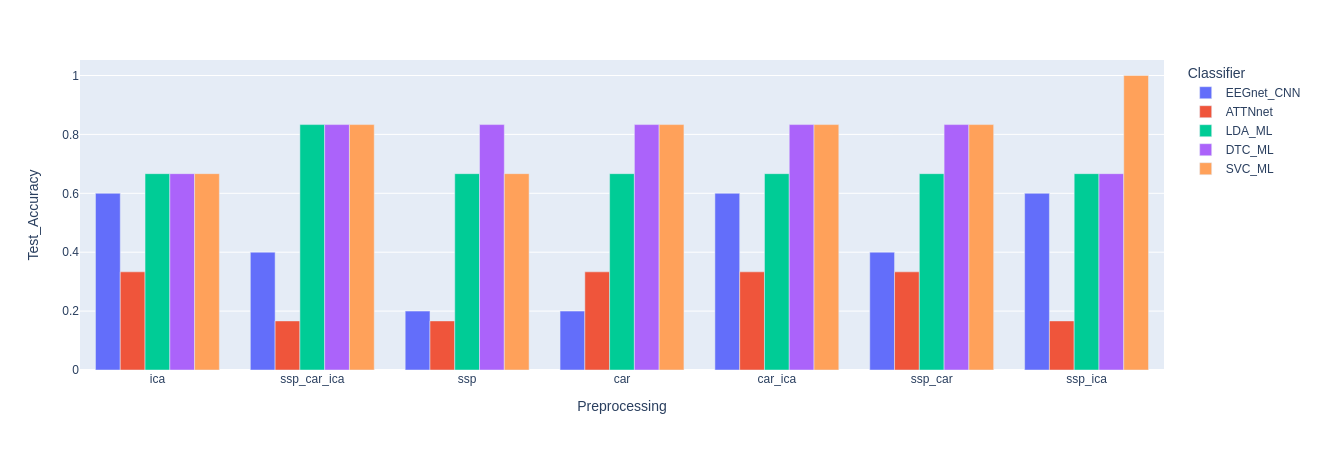
\includegraphics[width=1.0\textwidth]{images/preproc_test_acc_classifier_bar.png}
        \caption{Accuracy for different classification methods}
        \label{fig:preproc_test_acc_classifier}
        \end{center}
    \end{figure}

     \begin{figure}[H] 
     \begin{center}
        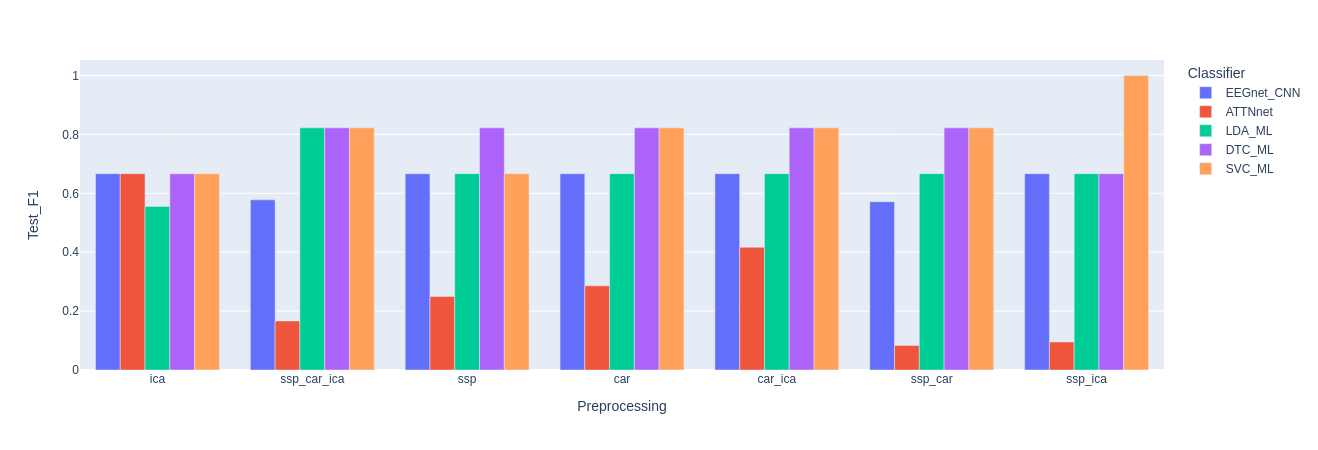
\includegraphics[width=1.0\textwidth]{images/preproc_test_f1_classifier_bar.png}
        \caption{F1 score for different classification methods}
        \label{fig:preproc_test_f1_classifier}
        \end{center}
    \end{figure}

The DTC and SVM classifiers provided the best accuracy for most preprocessing methods. EEGnet was able to perform better than ATTNnet as a classifier.

\section{Deep learning}
The Deep Learning methods used in analysing the brain signal requires individual evaluation as the networks have the ability to extract features and classify them. In some literatures, Deep Learning networks were used in only classification as the features were extracted from the EEG measurements before being fed into the network. Two networks \cite{2018_EEGNet} and \cite{2019_DLSTM_MI} are studied in this work and its results on data from OpenBCI headgear are analysed in the figures \ref{fig:preproc_test_f1_dl} and \ref{fig:preproc_test_acc_dl}.

     \begin{figure}[H] 
     \begin{center}
        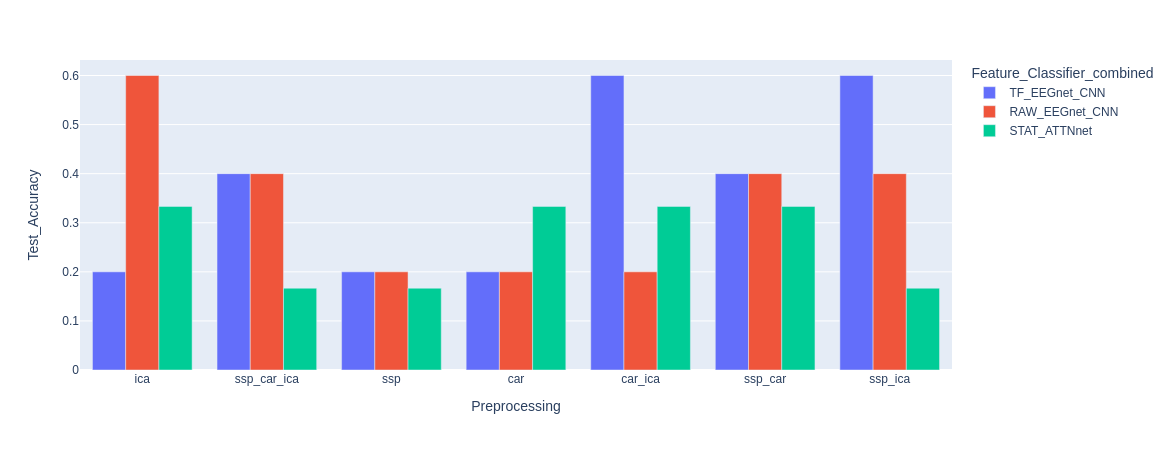
\includegraphics[width=1.0\textwidth]{images/preproc_test_acc_dl_bar.png}
        \caption{Accuracy: EEGnet versus ATTNnet}
        \label{fig:preproc_test_acc_dl}
        \end{center}
    \end{figure}

     \begin{figure}[H] 
     \begin{center}
        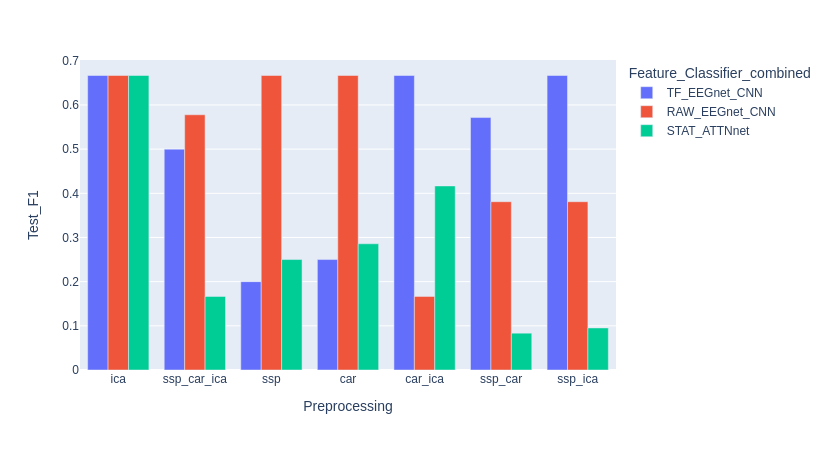
\includegraphics[width=1.0\textwidth]{images/preproc_test_f1_dl_bar.png}
        \caption{F1 score: EEGnet versus ATTNnet}
        \label{fig:preproc_test_f1_dl}
        \end{center}
    \end{figure}

EEGnet architecture can take both a scalogram image or the raw data as image and perform spatio-temporal analysis of the measured EEG data. ATTNnet is fed with several time-based statistical features to perform classification. The temporal information is remembered in the LSTMs in the architecture. The figures show that EEGnet provides best results with both TF image or a raw image as input.

\section{Time Analysis}
The time required for processing and classifying the information also play a crucial rule in deciding the best algorithm for controlling the steering in real time. The time information must also include the training time to incorporate portability to a different user or application. The figure \ref{fig:preproc_cv_time_feat} shows that ATTNnet takes the most time to train and validate the system. Generally all the deep learning methods take more time than the machine learning methods.
     \begin{figure}[H] 
     \begin{center}
        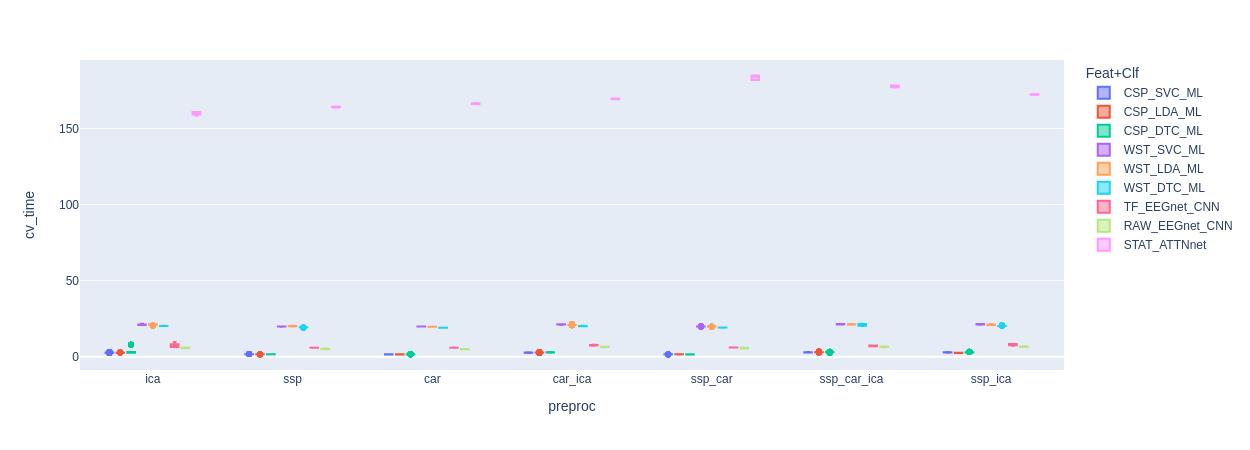
\includegraphics[width=1.0\textwidth]{images/preproc_cv_time_feat.png}
        \caption{Cross Validation time for different methods}
        \label{fig:preproc_cv_time_feat}
        \end{center}
    \end{figure}
    
The cross-validation time without the ATTNnet is given in figure \ref{fig:preproc_cv_time_feat2}.  EEGnet models using TF and Raw information require similar time, but WST methods require more time though they use the deep learning in its backend. CSP feature extraction method requires the least time and even less data to achieve results comparable to EEGnet models. 
     \begin{figure}[H] 
     \begin{center}
        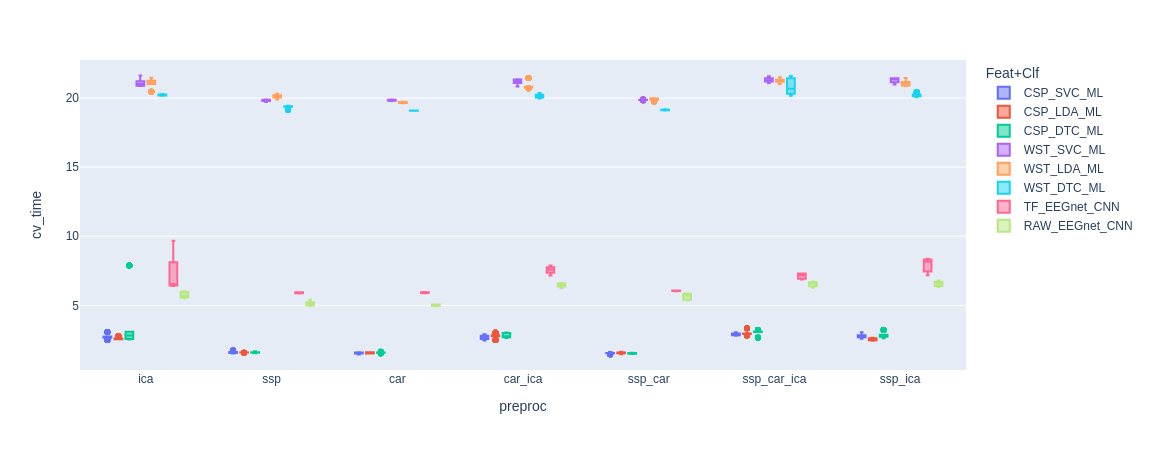
\includegraphics[width=1.0\textwidth]{images/preproc_cv_time_feat2.png}
        \caption{Cross Validation time for different methods (excluding ATTNnet)}
        \label{fig:preproc_cv_time_feat2}
        \end{center}
    \end{figure}
    
\section{Summary}
Based on the above analysis and different experiments, EEGnet model fed in with raw brain signal promises good accuracy in most scenarios. It is used in steering the simulated car in CARLA. During the training process, the training system helps in gathering event based epoched data which is used in training the EEGnet. While in testing and validation phase, the data from the BCI headgear had to be epoched for the same duration before being passed to EEGnet. The challenges faced in completing the task are discussed in the next chapter.